
\documentclass[10pt]{article}

\usepackage[a4paper,margin=0.65in]{geometry}
\usepackage{amsmath,amssymb}
\usepackage{graphicx}
\usepackage{booktabs}
\usepackage{array}
\usepackage{float}
\usepackage{hyperref}
\usepackage{enumitem}
\usepackage{xcolor}
\usepackage[font=small,labelfont=bf,skip=2pt]{caption}
\usepackage{tikz}
\usetikzlibrary{positioning,arrows.meta,shapes.geometric,fit,calc}

\setlist{nosep,leftmargin=*}
\renewcommand{\arraystretch}{1.2}
\setlength{\parindent}{0pt}
\setlength{\parskip}{2pt}

\tikzset{
layer/.style={
draw,
rounded corners,
minimum width=1.7cm,
minimum height=0.65cm,
align=center,
fill=blue!10,
font=\scriptsize
},
smalllayer/.style={
draw,
rounded corners,
minimum width=1.35cm,
minimum height=0.58cm,
align=center,
fill=green!10,
font=\scriptsize
},
arrow/.style={
-{Latex[length=2mm]},
thin
}
}

\newcommand{\figone}[4]{\begin{figure}[H]\centering\includegraphics[width=#2\linewidth]{#1}\caption{#3}\label{#4}\end{figure}}
\newcommand{\figtwo}[4]{\begin{figure}[H]\centering\includegraphics[width=0.485\linewidth]{#1}\hfill\includegraphics[width=0.485\linewidth]{#2}\caption{#3}\label{#4}\end{figure}}
\newcommand{\figthree}[5]{\begin{figure}[H]\centering\includegraphics[width=0.325\linewidth]{#1}\hfill\includegraphics[width=0.325\linewidth]{#2}\hfill\includegraphics[width=0.325\linewidth]{#3}\caption{#4}\label{#5}\end{figure}}
\newcommand{\result}[1]{\par\smallskip\noindent\fbox{\parbox{\dimexpr\linewidth-2\fboxsep-2\fboxrule\relax}{#1}}\par\smallskip}

\begin{document}

%%%%%%%%%%%%%%%%%%%%%%%%%%%%%%%%%%%%%%%%%%%%%%%%%%%%%%%%%%%%
% TITLE
%%%%%%%%%%%%%%%%%%%%%%%%%%%%%%%%%%%%%%%%%%%%%%%%%%%%%%%%%%%%

\begin{center}

{\large\textbf{Shiv Nadar University Chennai}}

\vspace{2mm}

{\normalsize\textbf{CS3807 -- Deep Learning Laboratory}}

\vspace{2mm}

{\large\textbf{Experiment 6}}

\vspace{1mm}

{\normalsize\textbf{End-to-End Study of RNN, LSTM and GRU for}}

{\normalsize\textbf{Sequence Learning and Video Understanding}}

\end{center}

\vspace{3mm}

\begin{tabular}{|p{3.4cm}|p{9.0cm}|p{1.4cm}|}
\hline
Degree \& Branch &
B.Tech Artificial Intelligence \& Data Science &
Semester V\\
\hline
Subject Code \& Name &
CS3807 -- Deep Learning Laboratory &
AY: 2026--27\\
\hline
\end{tabular}

%%%%%%%%%%%%%%%%%%%%%%%%%%%%%%%%%%%%%%%%%%%%%%%%%%%%%%%%%%%%
\section*{1. Objective}

The objective of this experiment is to develop an end-to-end understanding of
recurrent sequence learning by implementing and comparing Vanilla RNN, LSTM
and GRU models. The experiment also introduces Backpropagation Through Time
(BPTT), the limitations of conventional RNNs, and the use of CNN-extracted
features with recurrent networks for video understanding.

The experiment uses the UCI Human Activity Recognition Using Smartphones
dataset as the primary sequence dataset. Temporal input sequences are prepared and visualized, RNN/LSTM/GRU models are trained and compared, convergence and generalization are analysed, and the pipeline is extended
to video understanding using CNN feature extraction followed by an LSTM or
GRU.

A small synthetic sequence-to-sequence task is included at the end to
demonstrate the encoder--decoder framework.

%%%%%%%%%%%%%%%%%%%%%%%%%%%%%%%%%%%%%%%%%%%%%%%%%%%%%%%%%%%%
\section*{2. Learning Outcomes}

After completing this experiment, students will be able to:

\begin{itemize}
\item represent sequential data using the $(N,T,F)$ input format;
\item explain the architecture and operation of a Vanilla RNN;
\item explain Backpropagation Through Time and the vanishing/exploding gradient challenges;
\item implement sequence classification using SimpleRNN, LSTM and GRU;
\item compare RNN, LSTM and GRU using quantitative performance measures;
\item interpret training/validation curves and confusion matrices;
\item explain the role of CNNs in extracting spatial features from video frames;
\item construct a CNN--LSTM or CNN--GRU pipeline for video understanding;
\item explain the encoder--decoder architecture for sequence-to-sequence learning; and
\item draw conclusions using predictive performance, model complexity and computational cost.
\end{itemize}

%%%%%%%%%%%%%%%%%%%%%%%%%%%%%%%%%%%%%%%%%%%%%%%%%%%%%%%%%%%%
\section*{3. Dataset and Experimental Setup}

\textbf{Primary Dataset: UCI Human Activity Recognition Using Smartphones}

The UCI Human Activity Recognition (HAR) dataset contains smartphone sensor
measurements collected from subjects performing six activities:

\begin{itemize}
\item WALKING
\item WALKING\_UPSTAIRS
\item WALKING\_DOWNSTAIRS
\item SITTING
\item STANDING
\item LAYING
\end{itemize}

The experiment uses the raw inertial signal files rather than the
already-computed 561-feature vectors. Each activity window contains 128
temporal measurements. The three-axis body acceleration, three-axis
gyroscope and three-axis total acceleration signals provide nine channels.

Thus, the desired input representation is

\[
X\in\mathbb{R}^{N\times128\times9}.
\]

The dataset can be obtained from:

\url{https://archive.ics.uci.edu/dataset/240/human+activity+recognition+using+smartphones}

\subsection*{Expected Input}

For one sample:

\[
X_i\in\mathbb{R}^{128\times9}.
\]

For a batch of 32 samples:

\[
X_{\mathrm{batch}}\in\mathbb{R}^{32\times128\times9}.
\]

The dimensions represent:

\begin{center}
\begin{tabular}{|c|c|l|}
\hline
Dimension & Meaning & Value\\
\hline
$N$ & Number of sequences & 1976 (training)\\
$T$ & Time steps per sequence & 128\\
$F$ & Features/channels per time step & 9\\
\hline
\end{tabular}
\end{center}

Therefore, the model must receive a three-dimensional tensor rather than a
conventional two-dimensional tabular matrix.

%%%%%%%%%%%%%%%%%%%%%%%%%%%%%%%%%%%%%%%%%%%%%%%%%%%%%%%%%%%%
\section*{4. Overall Experimental Pipeline}

The complete sequence-classification pipeline is:

\begin{center}
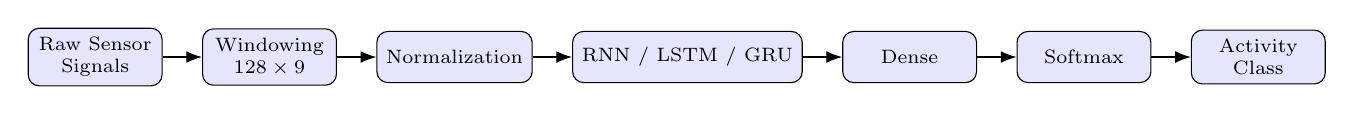
\begin{tikzpicture}[node distance=5mm]
\node[layer](a){Raw Sensor\\Signals};
\node[layer,right=of a](b){Windowing\\$128\times9$};
\node[layer,right=of b](c){Normalization};
\node[layer,right=of c](d){RNN / LSTM / GRU};
\node[layer,right=of d](e){Dense};
\node[layer,right=of e](f){Softmax};
\node[layer,right=of f](g){Activity\\Class};

\foreach \x/\y in {a/b,b/c,c/d,d/e,e/f,f/g}
\draw[arrow](\x)--(\y);
\end{tikzpicture}
\end{center}

The three recurrent models use the same input, output layer, optimizer,
batch size and evaluation protocol.

%%%%%%%%%%%%%%%%%%%%%%%%%%%%%%%%%%%%%%%%%%%%%%%%%%%%%%%%%%%%
\section*{5. Preprocessing}

Perform the following preprocessing steps:

\begin{enumerate}
\item Load the raw inertial signals.
\item Arrange every observation window as $128\times9$.
\item Assign one activity label to each window.
\item Encode the six activity labels.
\item Normalize the input using statistics calculated from the training data.
\item Create training, validation and test sets.
\item Verify the class distribution.
\end{enumerate}

\subsection*{Preprocessing Output}

\result{\textbf{Observed output (this run).}
\begin{center}\ttfamily\small
\begin{tabular}{l}
Input tensor shape:\\
Training~~~:~(1976,~128,~9)\\
Validation~:~(424,~~128,~9)\\
Testing~~~~:~(2947,~128,~9)\\[2pt]
Number of classes: 6\\
Number of features per time step: 9\\
Sequence length: 128
\end{tabular}
\end{center}
A class-balanced subset of 2400 windows was drawn from the 7352-window official training partition and split (stratified) into 1976 training and 424 validation windows. The complete official test partition (2947 windows) was retained as the test set. Each channel was z-score normalized with training-set statistics (verified: training per-channel mean $=0$, standard deviation $=1$). The class distribution is:
\begin{center}
\begin{tabular}{|l|c|c|c|}
\hline
Class & Train & Validation & Test\\
\hline
WALKING & 330 & 70 & 496\\
WALKING\_UPSTAIRS & 330 & 70 & 471\\
WALKING\_DOWNSTAIRS & 329 & 71 & 420\\
SITTING & 329 & 71 & 491\\
STANDING & 329 & 71 & 532\\
LAYING & 329 & 71 & 537\\
\hline
\end{tabular}
\end{center}}

%%%%%%%%%%%%%%%%%%%%%%%%%%%%%%%%%%%%%%%%%%%%%%%%%%%%%%%%%%%%
\section*{6. Temporal Data Visualization}

One representative window from each of three activity classes (WALKING, SITTING and LAYING) is plotted for three channels (body acceleration $x$, body gyroscope $x$ and total acceleration $x$).

\textbf{Plot 1: Sensor signal versus time}

\figone{images/plot1_temporal_signals.png}{0.78}{Plot 1: sensor value versus time step for one representative window each of WALKING, SITTING and LAYING (channels: body\_acc\_x, body\_gyro\_x, total\_acc\_x). Note that the y-axis range differs between panels.}{fig:plot1}

\result{\textbf{Inference (Plot 1).}
\textit{Pattern:} WALKING shows large, irregular quasi-periodic oscillations on all three channels (total\_acc\_x roughly $0.5$--$1.8$, body\_gyro\_x down to about $-1.4$), whereas SITTING is almost flat: total\_acc\_x stays near $1.0$ (the gravity component) and the body-acceleration and gyroscope channels stay near $0$. LAYING is also low-amplitude (values within about $\pm0.07$) but its gravity component on the x-axis sits near $0.04$ instead of $1.0$.
\textit{Similar activities:} the static postures (SITTING, LAYING, and STANDING, which is not plotted) are all low-variance signals that differ mainly in the constant gravity offset, i.e. the orientation of the phone; this is consistent with the SITTING/STANDING confusion seen later in the confusion matrices.
\textit{Why order matters:} in WALKING the peaks of the accelerometer and gyroscope channels are phase-related and repeat with a gait rhythm; shuffling the 128 time steps would keep the amplitude statistics but destroy this phase and periodicity information, which is exactly what a recurrent model exploits.}

%%%%%%%%%%%%%%%%%%%%%%%%%%%%%%%%%%%%%%%%%%%%%%%%%%%%%%%%%%%%
\section*{7. Vanilla RNN Architecture}

A Vanilla RNN maintains a hidden state that is updated at every time step:

\[
h_t=\tanh(W_xx_t+W_hh_{t-1}+b_h).
\]

The output can be written as

\[
y_t=g(W_yh_t+b_y).
\]

For sequence classification, the final hidden representation can be passed
to a classifier.

\begin{center}
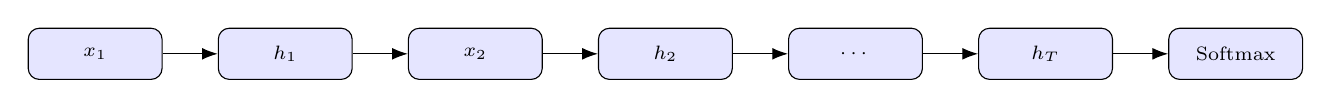
\begin{tikzpicture}[node distance=7mm]
\node[layer](x1){$x_1$};
\node[layer,right=of x1](h1){$h_1$};
\node[layer,right=of h1](x2){$x_2$};
\node[layer,right=of x2](h2){$h_2$};
\node[layer,right=of h2](x3){$\cdots$};
\node[layer,right=of x3](h3){$h_T$};
\node[layer,right=of h3](y){Softmax};

\draw[arrow](x1)--(h1);
\draw[arrow](h1)--(x2);
\draw[arrow](x2)--(h2);
\draw[arrow](h2)--(x3);
\draw[arrow](x3)--(h3);
\draw[arrow](h3)--(y);
\end{tikzpicture}
\end{center}

The diagram represents the unrolled view of an RNN. The same recurrent weights
are reused across time steps.

%%%%%%%%%%%%%%%%%%%%%%%%%%%%%%%%%%%%%%%%%%%%%%%%%%%%%%%%%%%%
\section*{8. Backpropagation Through Time}

When an RNN is unrolled, the loss depends on the sequence of hidden states.
Backpropagation Through Time (BPTT) propagates the error backward through
the recurrent steps.

\begin{center}
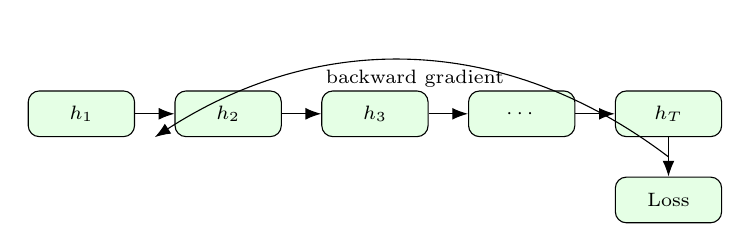
\begin{tikzpicture}[node distance=5mm]
\node[smalllayer](a){$h_1$};
\node[smalllayer,right=of a](b){$h_2$};
\node[smalllayer,right=of b](c){$h_3$};
\node[smalllayer,right=of c](d){$\cdots$};
\node[smalllayer,right=of d](e){$h_T$};
\node[smalllayer,below=of e](l){Loss};

\draw[arrow](a)--(b);
\draw[arrow](b)--(c);
\draw[arrow](c)--(d);
\draw[arrow](d)--(e);
\draw[arrow](e)--(l);

\draw[arrow]($(e.south)!0.5!(l.north)$) to[bend right=35]
node[below,font=\scriptsize]{backward gradient} ($(a.south)!0.5!(b.south)$);
\end{tikzpicture}
\end{center}

Repeated multiplication of derivatives through many time steps can cause
gradients to become extremely small or extremely large.

\subsection*{Challenges}

\begin{itemize}
\item Vanishing gradients
\item Exploding gradients
\item Difficulty learning long-term dependencies
\item Sequential computation and limited parallelism
\end{itemize}

The vanishing-gradient problem can be conceptually represented as

\[
\left|\frac{\partial h_t}{\partial h_{t-k}}\right|\rightarrow0
\]

while exploding gradients correspond to very large gradient magnitudes.

\subsection*{Numerical Exercise}

Consider

\[
x_1=0.5,\qquad x_2=0.7,\qquad x_3=0.2,
\]

\[
h_0=0,\qquad W_x=0.5,\qquad W_h=0.8,\qquad b=0.1.
\]

Using

\[
h_t=\tanh(W_xx_t+W_hh_{t-1}+b),
\]

calculate $h_1$, $h_2$ and $h_3$ manually.

\result{\textbf{Worked solution and program check.}
\[
h_1=\tanh(0.5\cdot0.5+0.8\cdot0+0.1)=\tanh(0.35)=0.3364,
\]
\[
h_2=\tanh(0.5\cdot0.7+0.8\cdot0.3364+0.1)=\tanh(0.7191)=0.6164,
\]
\[
h_3=\tanh(0.5\cdot0.2+0.8\cdot0.6164+0.1)=\tanh(0.6931)=0.6000.
\]
\begin{center}
\begin{tabular}{|c|c|c|}
\hline
State & Manual / NumPy & Keras \texttt{SimpleRNNCell}\\
\hline
$h_1$ & 0.336376 & 0.336376\\
$h_2$ & 0.616352 & 0.616352\\
$h_3$ & 0.599958 & 0.599958\\
\hline
\end{tabular}
\end{center}
The hand calculation, the NumPy program and the Keras cell agree to six decimal places. The hidden state stays bounded in $(-1,1)$ because of $\tanh$, and $h_3$ is still strongly influenced by $x_2$ through $W_hh_2$, illustrating how information flows forward through the recurrence.}

%%%%%%%%%%%%%%%%%%%%%%%%%%%%%%%%%%%%%%%%%%%%%%%%%%%%%%%%%%%%
\section*{9. RNN Implementation}

A small recurrent architecture is used:

\begin{center}
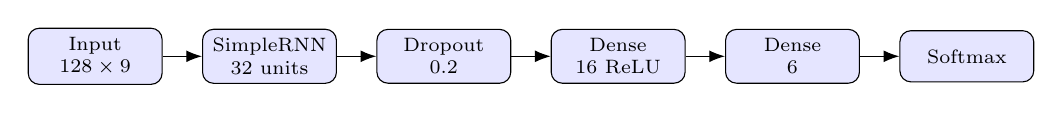
\begin{tikzpicture}[node distance=5mm]
\node[layer](a){Input\\$128\times9$};
\node[layer,right=of a](b){SimpleRNN\\32 units};
\node[layer,right=of b](c){Dropout\\0.2};
\node[layer,right=of c](d){Dense\\16 ReLU};
\node[layer,right=of d](e){Dense\\6};
\node[layer,right=of e](f){Softmax};

\foreach \x/\y in {a/b,b/c,c/d,d/e,e/f}
\draw[arrow](\x)--(\y);
\end{tikzpicture}
\end{center}

\textbf{Training configuration:}

\begin{center}
\begin{tabular}{|l|l|}
\hline
Parameter & Value\\
\hline
Recurrent units & 32\\
Dropout & 0.2\\
Optimizer & Adam\\
Learning rate & $10^{-3}$\\
Batch size & 32\\
Epochs & 30\\
Loss & Sparse categorical cross-entropy\\
\hline
\end{tabular}
\end{center}

\result{\textbf{Observed model summary (RNN).}
SimpleRNN(32): $32(9+32)+32=1{,}344$ parameters; Dense(16): $528$; Dense(6): $102$; total \textbf{1,974} trainable parameters. Training used the CPU (no GPU was available).}

%%%%%%%%%%%%%%%%%%%%%%%%%%%%%%%%%%%%%%%%%%%%%%%%%%%%%%%%%%%%
\section*{10. LSTM Architecture}

LSTM introduces a memory cell and gates to control information flow.

The forget gate is

\[
f_t=\sigma(W_f[h_{t-1},x_t]+b_f),
\]

the input gate is

\[
i_t=\sigma(W_i[h_{t-1},x_t]+b_i),
\]

and the output gate is

\[
o_t=\sigma(W_o[h_{t-1},x_t]+b_o).
\]

The candidate cell state is

\[
\tilde{C}_t=
\tanh(W_C[h_{t-1},x_t]+b_C),
\]

and the cell state is

\[
C_t=f_tC_{t-1}+i_t\tilde{C}_t.
\]

The hidden state is

\[
h_t=o_t\tanh(C_t).
\]

\begin{center}
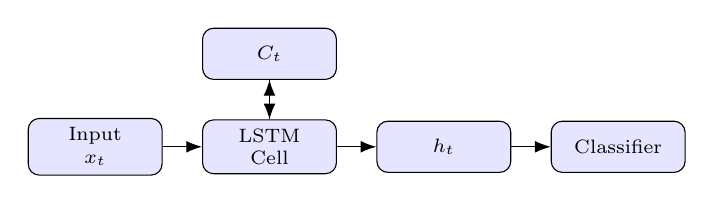
\begin{tikzpicture}[node distance=5mm]
\node[layer](a){Input\\$x_t$};
\node[layer,right=of a](b){LSTM\\Cell};
\node[layer,right=of b](c){$h_t$};
\node[layer,above=of b](d){$C_t$};
\node[layer,right=of c](e){Classifier};

\draw[arrow](a)--(b);
\draw[arrow](b)--(c);
\draw[arrow](b)--(d);
\draw[arrow](c)--(e);
\draw[arrow](d)--(b);
\end{tikzpicture}
\end{center}

\result{\textbf{Inference.} The cell state is updated additively, $C_t=f_tC_{t-1}+i_t\tilde{C}_t$, so when the forget gate is close to 1 and the input gate close to 0 the memory, and its gradient $\partial C_t/\partial C_{t-1}=\mathrm{diag}(f_t)$, pass through many time steps essentially unchanged, instead of being squashed by a $\tanh$ and multiplied by $W_h$ at every step as in a vanilla RNN. The forget gate erases irrelevant memory, the input gate selects which new information is written, and the output gate controls how much of the memory is exposed as $h_t$. This gated additive path is why the LSTM (89.2\% test macro F1) far outperforms the vanilla RNN (68.0\%) on 128-step sequences.}

%%%%%%%%%%%%%%%%%%%%%%%%%%%%%%%%%%%%%%%%%%%%%%%%%%%%%%%%%%%%
\section*{11. GRU Architecture}

GRU uses two principal gates:

\[
z_t=\sigma(W_z[h_{t-1},x_t]+b_z)
\]

and

\[
r_t=\sigma(W_r[h_{t-1},x_t]+b_r).
\]

The candidate hidden state is

\[
\tilde{h}_t=
\tanh(W_h[r_t\odot h_{t-1},x_t]+b_h).
\]

The hidden state is updated using

\[
h_t=(1-z_t)h_{t-1}+z_t\tilde{h}_t.
\]

\begin{center}
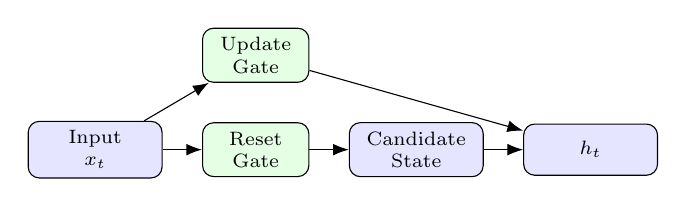
\begin{tikzpicture}[node distance=5mm]
\node[layer](a){Input\\$x_t$};
\node[smalllayer,right=of a](b){Reset\\Gate};
\node[smalllayer,above=of b](c){Update\\Gate};
\node[layer,right=of b](d){Candidate\\State};
\node[layer,right=of d](e){$h_t$};

\draw[arrow](a)--(b);
\draw[arrow](a)--(c);
\draw[arrow](b)--(d);
\draw[arrow](c)--(e);
\draw[arrow](d)--(e);
\end{tikzpicture}
\end{center}

\result{\textbf{Inference.} The vanilla RNN has no gates and a single state $h_t$; the LSTM has three gates (forget, input, output) and two states ($h_t$ and $C_t$); the GRU has two gates (update, reset) and a single state $h_t$, obtained by merging the cell and hidden states. The GRU thus keeps an additive, gated path ($h_t=(1-z_t)h_{t-1}+z_t\tilde{h}_t$) with fewer parameters than the LSTM (4,128 vs 5,376 in the recurrent layer for 32 units).}

%%%%%%%%%%%%%%%%%%%%%%%%%%%%%%%%%%%%%%%%%%%%%%%%%%%%%%%%%%%%
\section*{12. LSTM and GRU Implementation}

The same classifier as for the RNN is used, replacing only the recurrent
layer.

\begin{center}
\begin{tabular}{|l|c|c|c|}
\hline
Model & Recurrent Layer & Units & Output Classes\\
\hline
RNN & SimpleRNN & 32 & 6\\
LSTM & LSTM & 32 & 6\\
GRU & GRU & 32 & 6\\
\hline
\end{tabular}
\end{center}

All other experimental conditions remain unchanged.

\result{\textbf{Observed parameter counts.}
With $9$ inputs and $32$ units, one recurrent gate/candidate block has $32(9+32)+32=1{,}344$ parameters (the Keras GRU with \texttt{reset\_after} uses two bias vectors, giving $32\cdot9+32\cdot32+2\cdot32=1{,}376$ per block). The classifier head (Dense 16 and Dense 6) adds $630$. Therefore:
\begin{center}
\begin{tabular}{|l|c|c|c|}
\hline
Model & Recurrent-layer parameters & Head & Total\\
\hline
RNN (1 block) & 1,344 & 630 & 1,974\\
LSTM (4 blocks) & 5,376 & 630 & 6,006\\
GRU (3 blocks) & 4,128 & 630 & 4,758\\
\hline
\end{tabular}
\end{center}}

%%%%%%%%%%%%%%%%%%%%%%%%%%%%%%%%%%%%%%%%%%%%%%%%%%%%%%%%%%%%
\section*{13. Training Plots}

Training and validation loss (Plot 2) and accuracy (Plot 3) are plotted against the epoch for each of the RNN, LSTM and GRU.

\figtwo{images/plot2_rnn_loss.png}{images/plot3_rnn_accuracy.png}{Plots 2 and 3, RNN: training/validation loss (left) and accuracy (right) over 30 epochs.}{fig:rnncurves}
\figtwo{images/plot2_lstm_loss.png}{images/plot3_lstm_accuracy.png}{Plots 2 and 3, LSTM: training/validation loss (left) and accuracy (right) over 30 epochs.}{fig:lstmcurves}
\figtwo{images/plot2_gru_loss.png}{images/plot3_gru_accuracy.png}{Plots 2 and 3, GRU: training/validation loss (left) and accuracy (right) over 30 epochs.}{fig:grucurves}

\result{\textbf{Observed convergence statistics (epoch 30 unless stated).}
\begin{center}
\begin{tabular}{|l|c|c|c|c|c|}
\hline
Model & Train acc. (\%) & Val acc. (\%) & Gap (pts) & Min val loss (epoch) & Final val loss\\
\hline
RNN & 76.8 & 70.3 & 6.5 & 0.584 (17) & 0.638\\
LSTM & 96.1 & 94.3 & 1.7 & 0.129 (17) & 0.140\\
GRU & 96.1 & 92.7 & 3.4 & 0.130 (24) & 0.136\\
\hline
\end{tabular}
\end{center}
\textbf{RNN.} Training accuracy climbs from 40.9\% to 76.8\% and validation accuracy from 53.1\% to 70.3\%, but the curves are unstable (validation accuracy falls from 72.9\% at epoch 24 to 64.1\% at epoch 25) and have not converged after 30 epochs. Because even the \emph{training} accuracy stays near 77\%, the dominant problem is underfitting or optimisation difficulty rather than overfitting, consistent with the difficulty of propagating gradients over 128 steps and with the small capacity (1,974 parameters). The validation loss reaches its minimum at epoch 17 and then rises slightly (0.584 to 0.638), a mild sign of overfitting late in training.
\textbf{LSTM.} Training and validation accuracy reach 96.1\% and 94.3\% with a 1.7-point gap; validation loss is lowest at epoch 17 (0.129) and ends slightly higher (0.140) while training loss keeps decreasing (0.112), so convergence is essentially reached by epoch 17--20 and further training only adds a small overfitting component.
\textbf{GRU.} Training accuracy is again 96.1\% with 92.7\% validation accuracy (gap 3.4 points); the validation loss minimum (0.130) occurs later, at epoch 24, and ends at 0.136. The GRU therefore converges to a similar loss level as the LSTM with a somewhat larger accuracy gap.
\textbf{Generalization gap.} The validation windows are drawn at random from the same pool as the training windows (no subject-wise split) and consecutive HAR windows overlap by 50\%, so validation accuracy is likely optimistic: the subject-independent test accuracies (89.1\% LSTM, 89.5\% GRU) are 3--5 points lower, whereas the RNN, which underfits, shows almost no drop (70.3\% to 69.3\%).}

%%%%%%%%%%%%%%%%%%%%%%%%%%%%%%%%%%%%%%%%%%%%%%%%%%%%%%%%%%%%
\section*{14. Performance Evaluation}

Each model is evaluated on the independent test set using the following metrics:

\begin{itemize}
\item Accuracy
\item Precision
\item Recall
\item F1-score
\item Confusion matrix
\item Number of trainable parameters
\item Training time
\end{itemize}

For multi-class classification, macro-averaged Precision, Recall and
F1-score are reported.

\begin{center}
\begin{tabular}{|l|c|c|c|}
\hline
Metric & RNN & LSTM & GRU\\
\hline
Accuracy (\%) & 69.29 & 89.11 & 89.55\\
Macro Precision (\%) & 68.99 & 89.11 & 89.55\\
Macro Recall (\%) & 68.49 & 89.30 & 89.70\\
Macro F1 (\%) & 68.02 & 89.16 & 89.50\\
Parameters & 1,974 & 6,006 & 4,758\\
Training Time (s) & 46.1 & 95.9 & 121.6\\
\hline
\end{tabular}
\end{center}

All metrics are computed on the independent test set of 2947 windows. Training times are wall-clock seconds on CPU for 30 epochs.

%%%%%%%%%%%%%%%%%%%%%%%%%%%%%%%%%%%%%%%%%%%%%%%%%%%%%%%%%%%%
\section*{15. Confusion Matrix Analysis}

\textbf{Plot 4: Confusion Matrix}

A separate confusion matrix is generated for each model.

\figthree{images/plot4_rnn_confusion.png}{images/plot4_lstm_confusion.png}{images/plot4_gru_confusion.png}{Plot 4: test-set confusion matrices for RNN (left), LSTM (centre) and GRU (right); rows are actual classes and columns are predicted classes.}{fig:cms}

\result{\textbf{Observed per-class recall on the test set (\%).}
\begin{center}
\begin{tabular}{|l|c|c|c|}
\hline
Class & RNN & LSTM & GRU\\
\hline
WALKING & 32.9 & 94.0 & 91.1\\
WALKING\_UPSTAIRS & 61.8 & 92.8 & 91.7\\
WALKING\_DOWNSTAIRS & 65.0 & 96.0 & 97.1\\
SITTING & 65.0 & 76.6 & 76.6\\
STANDING & 91.4 & 81.6 & 86.7\\
LAYING & 95.0 & 95.0 & 95.0\\
\hline
\end{tabular}
\end{center}
\textbf{Highest recognition rate:} LAYING for the RNN (95.0\%), WALKING\_DOWNSTAIRS for the LSTM (96.0\%) and the GRU (97.1\%); LAYING is 95.0\% for all three models.
\textbf{Largest number of misclassifications:} WALKING for the RNN (333 of 496 windows wrong, mostly assigned to WALKING\_UPSTAIRS (192) and WALKING\_DOWNSTAIRS (122)); SITTING for both the LSTM and the GRU (115 of 491 wrong).
\textbf{Frequently confused pairs:} SITTING$\leftrightarrow$STANDING is the dominant confusion for all models (LSTM: 104 SITTING predicted as STANDING and 95 the reverse; GRU: 91 and 70; RNN: 166 and 40). For the RNN the three walking classes are also heavily mixed with one another; in the LSTM and GRU these walking-class errors shrink to at most 43 windows per cell.
\textbf{Consistency across models:} the SITTING/STANDING confusion and the LAYING$\rightarrow$WALKING\_UPSTAIRS errors (25 for the RNN, 27 for both LSTM and GRU) persist in every model, so they are unlikely to be caused by recurrent-cell choice alone; a plausible (untested) explanation is that static postures differ only by a small gravity-direction offset (Plot 1) and that some test subjects hold the phone in atypical orientations. The gated models remove most of the walking-class errors that the vanilla RNN makes.}

%%%%%%%%%%%%%%%%%%%%%%%%%%%%%%%%%%%%%%%%%%%%%%%%%%%%%%%%%%%%
\section*{16. RNN vs. LSTM vs. GRU Comparison}

The three models are compared below.

\begin{center}
\begin{tabular}{|l|c|c|c|}
\hline
Property & RNN & LSTM & GRU\\
\hline
Hidden state & Yes & Yes & Yes\\
Cell state & No & Yes & No\\
Forget gate & No & Yes & No\\
Input gate & No & Yes & No\\
Output gate & No & Yes & No\\
Update gate & No & No & Yes\\
Reset gate & No & No & Yes\\
Parameters & 1,974 & 6,006 & 4,758\\
Training time (s) & 46.1 & 95.9 & 121.6\\
Test F1-score (\%) & 68.02 & 89.16 & 89.50\\
\hline
\end{tabular}
\end{center}

\textbf{Plot 5: Model Performance Comparison}

Test Accuracy and Macro F1-score are compared with normalized computational measures.

\figone{images/plot5_model_comparison.png}{0.62}{Plot 5: test accuracy and macro F1 (as fractions), with min--max normalized parameter count and training time. Because of the min--max scaling, the RNN bars for parameters and time are zero by construction, not because its cost is zero.}{fig:plot5}

\textbf{Trade-off among:}

\[
\text{Predictive Performance}
\quad\leftrightarrow\quad
\text{Model Complexity}
\quad\leftrightarrow\quad
\text{Training Cost}.
\]

\result{\textbf{Inference (Plots 4--5 and the table above).}
Moving from the vanilla RNN to a gated cell raises test macro F1 by about 21 points in the seed-42 run (68.0\% $\to$ 89.2\% LSTM / 89.5\% GRU); over three seeds (Section~27, Exercise~1) the RNN averages $72.9\pm7.0$\% against $89.3\pm1.0$\% (LSTM) and $89.9\pm0.4$\% (GRU), so the gain is about 16--17 points and the seed-42 RNN run lies at the low end of a very unstable distribution at the price of $3.0\times$ (LSTM) or $2.4\times$ (GRU) more parameters and roughly $2$--$2.6\times$ the wall-clock training time. The GRU is $20.8\%$ smaller than the LSTM (4,758 vs 6,006 parameters) yet scores marginally higher (+0.33 F1, +0.44 accuracy); with a single seed per model and a seed-to-seed standard deviation of about 0.4--1.0 F1 points for the gated cells (Section~27), this difference should be regarded as \emph{no measurable difference}, not as a GRU advantage. The GRU's longer measured training time (121.6 s vs 95.9 s) contradicts the expectation that fewer parameters mean faster training. An earlier reading attributed this to session effects, but the controlled benchmark and the three-seed runs of Section~27 show the GRU to be consistently 1.25--1.45$\times$ slower than the LSTM in this Keras/CPU setup; the cause was not profiled and it may not carry over to other hardware or backends. Overall, the large performance gain comes from introducing gating, whereas the choice between LSTM and GRU is nearly free in accuracy terms and modest in cost terms.}

%%%%%%%%%%%%%%%%%%%%%%%%%%%%%%%%%%%%%%%%%%%%%%%%%%%%%%%%%%%%
\section*{17. Effect of Sequence Length}

To study the effect of temporal context, the experiment is repeated for the sequence lengths

\[
T\in\{32,64,128\}.
\]

\begin{center}
\begin{tabular}{|c|c|c|c|}
\hline
Sequence Length & RNN F1 & LSTM F1 & GRU F1\\
\hline
32 & 70.83 & 86.43 & 86.80\\
64 & 69.63 & 91.56 & 89.79\\
128 & 67.68 & 89.51 & 89.32\\
\hline
\end{tabular}
\end{center}

Shorter sequences were obtained by keeping the first $T$ time steps of each normalized window ($T=32,64,128$ correspond to about $0.64$, $1.28$ and $2.56$ s of signal at 50 Hz). Values are test macro F1 (\%).

\textbf{Plot 6: Sequence Length vs. Test F1-score}

\figone{images/plot6_seqlen_vs_f1.png}{0.55}{Plot 6: test macro F1 versus sequence length $T$ for RNN, LSTM and GRU.}{fig:plot6}

\result{\textbf{Inference (Plot 6).}
\textit{RNN:} F1 decreases as the sequence gets longer (70.8 $\to$ 69.6 $\to$ 67.7). This is consistent with gradients from early time steps not being propagated through a long unrolled tanh recurrence, but it is \emph{not} established by these runs: the RNN's seed-to-seed standard deviation is about 7 F1 points (Section~27), more than twice the 3.2-point trend, so the single-seed trend could be noise. \textit{LSTM and GRU:} both improve substantially from $T{=}32$ to $T{=}64$ (LSTM +5.1 points, GRU +3.0 points), showing that 0.64 s of signal is too short to characterise an activity and that additional context is useful; between $T{=}64$ and $T{=}128$ the F1 changes by $-2.0$ (LSTM) and $-0.5$ (GRU) points. Whether that small decrease is real cannot be concluded from one seed: the LSTM's and GRU's seed-to-seed standard deviations are about 1.0 and 0.4 F1 points (Section~27), so the $-2.0$ (LSTM) is suggestive at most and the $-0.5$ (GRU) is noise, whereas the $32\to64$ gains of the gated models (+5.1, +3.0) are several standard deviations and are credible. Note also that shorter windows reduce the cost per epoch, so $T$ trades context for computation.}

%%%%%%%%%%%%%%%%%%%%%%%%%%%%%%%%%%%%%%%%%%%%%%%%%%%%%%%%%%%%
\section*{18. Video Understanding Using CNN and RNN}

This part demonstrates the application:

\[
\boxed{\text{Video Understanding using CNN + RNN}}
\]

A video is a sequence of image frames. CNNs are used to extract spatial
features from individual frames, while RNN/LSTM/GRU models the temporal
relationship among those features.

The complete pipeline is:

\begin{center}
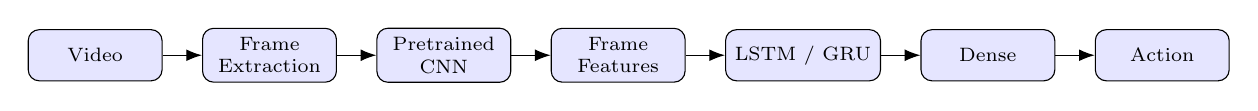
\begin{tikzpicture}[node distance=5mm]
\node[layer](a){Video};
\node[layer,right=of a](b){Frame\\Extraction};
\node[layer,right=of b](c){Pretrained\\CNN};
\node[layer,right=of c](d){Frame\\Features};
\node[layer,right=of d](e){LSTM / GRU};
\node[layer,right=of e](f){Dense};
\node[layer,right=of f](g){Action};

\foreach \x/\y in {a/b,b/c,c/d,d/e,e/f,f/g}
\draw[arrow](\x)--(\y);
\end{tikzpicture}
\end{center}

\subsection*{Dataset}

A small subset of the UCF101 action-recognition dataset is used:

\url{https://www.crcv.ucf.edu/data/UCF101.php}

Five action classes with eight videos per class (40 videos in total) are used:

\begin{itemize}
\item Basketball
\item Biking
\item WalkingWithDog
\item JumpingJack
\item TennisSwing
\end{itemize}

%%%%%%%%%%%%%%%%%%%%%%%%%%%%%%%%%%%%%%%%%%%%%%%%%%%%%%%%%%%%
\section*{19. Expected Video Input and Output}

Ten frames are sampled uniformly from each video.

Each frame is resized to

\[
224\times224\times3.
\]

A pretrained CNN such as MobileNetV2 is used only as a feature extractor.

If the CNN produces a feature vector of dimension $D$, then the recurrent
network receives:

\[
X\in\mathbb{R}^{10\times D}.
\]

For a batch of $B$ videos:

\[
X\in\mathbb{R}^{B\times10\times D}.
\]

The output is a probability vector over the selected action classes.

\result{\textbf{Observed setup and output (this run).}
Five UCF101 classes were used: Basketball, Biking, WalkingWithDog, JumpingJack and TennisSwing, with 8 videos per class (40 videos in total). Ten frames were sampled uniformly from every video and resized to $224\times224\times3$. The video-level split is stratified: 25 training, 7 validation and 8 test videos. The CNN feature tensor is $(40,10,1280)$, i.e. $D=1280$. Example prediction from the CNN--LSTM (test video \texttt{v\_BasketballDunk\_g13\_c04}, softmax confidence taken from the trained model):
\begin{center}\ttfamily\small
\begin{tabular}{l}
Predicted~class~:~Basketball\\
Actual~class~~~~:~Basketball\\
Confidence~~~~~~:~0.94
\end{tabular}
\end{center}}

%%%%%%%%%%%%%%%%%%%%%%%%%%%%%%%%%%%%%%%%%%%%%%%%%%%%%%%%%%%%
\section*{20. CNN Feature Extraction}

A pretrained CNN with the classification head removed is used.

\begin{center}
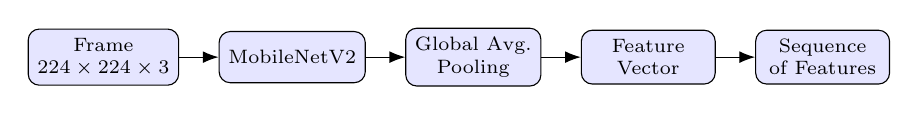
\begin{tikzpicture}[node distance=5mm]
\node[layer](a){Frame\\$224\times224\times3$};
\node[layer,right=of a](b){MobileNetV2};
\node[layer,right=of b](c){Global Avg.\\Pooling};
\node[layer,right=of c](d){Feature\\Vector};
\node[layer,right=of d](e){Sequence\\of Features};

\foreach \x/\y in {a/b,b/c,c/d,d/e}
\draw[arrow](\x)--(\y);
\end{tikzpicture}
\end{center}

The pretrained CNN is frozen and used to extract features first; the recurrent classifier is then trained on these features.



\result{\textbf{Observation.} The frozen MobileNetV2 with global average pooling produces a feature dimension of $D=1280$ per frame. The tensor supplied to the recurrent network is $(B,10,1280)$: $(25,10,1280)$ for training, $(7,10,1280)$ for validation and $(8,10,1280)$ for testing.}

%%%%%%%%%%%%%%%%%%%%%%%%%%%%%%%%%%%%%%%%%%%%%%%%%%%%%%%%%%%%
\section*{21. CNN--LSTM / CNN--GRU Model}

The following architecture is used:

\begin{center}
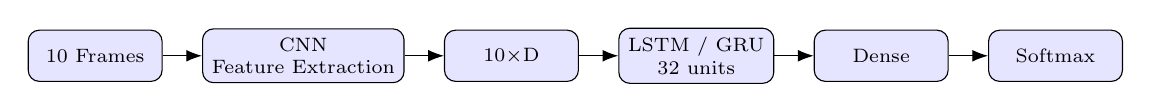
\begin{tikzpicture}[node distance=5mm]
\node[layer](a){10 Frames};
\node[layer,right=of a](b){CNN\\Feature Extraction};
\node[layer,right=of b](c){10$\times$D};
\node[layer,right=of c](d){LSTM / GRU\\32 units};
\node[layer,right=of d](e){Dense};
\node[layer,right=of e](f){Softmax};

\foreach \x/\y in {a/b,b/c,c/d,d/e,e/f}
\draw[arrow](\x)--(\y);
\end{tikzpicture}
\end{center}

\textbf{Plot 7: Video Sample Frames}

\figone{images/plot7_video_frames_corrected.png}{1.0}{Plot 7: ten uniformly sampled frames (t=0--9) from a Basketball video (UCF101, \texttt{v\_BasketballDunk\_g04\_c03}), as supplied to the CNN.}{fig:plot7}

\textbf{Plot 8: Video Training and Validation Curves}

\figtwo{images/plot2_cnn_lstm_loss.png}{images/plot3_cnn_lstm_accuracy.png}{Plot 8a, CNN--LSTM: training/validation loss (left) and accuracy (right) over 20 epochs.}{fig:cnnlstmcurves}
\figtwo{images/plot2_cnn_gru_loss.png}{images/plot3_cnn_gru_accuracy.png}{Plot 8b, CNN--GRU: training/validation loss (left) and accuracy (right) over 20 epochs.}{fig:cnngrucurves}

\textbf{Plot 9: Video Confusion Matrix}

\figtwo{images/plot9_cnn_lstm_video_confusion.png}{images/plot9_cnn_gru_video_confusion_corrected.png}{Plot 9: video test-set confusion matrices for CNN--LSTM (left) and CNN--GRU (right); 8 test videos in total.}{fig:videocm}

\result{\textbf{Observed video results (test set of 8 videos).}
\begin{center}
\begin{tabular}{|l|c|c|c|c|c|c|}
\hline
Model & Acc. (\%) & Prec. (\%) & Rec. (\%) & F1 (\%) & Parameters & Time (s)\\
\hline
CNN--LSTM & 100.00 & 100.00 & 100.00 & 100.00 & 168,229 & 8.3\\
CNN--GRU & 87.50 & 93.33 & 90.00 & 89.33 & 126,309 & 8.3\\
\hline
\end{tabular}
\end{center}
Per-video predictions (softmax confidence in the Conf.\ columns):
\begin{center}
\small
\begin{tabular}{|l|l|c|l|c|}
\hline
Actual (video) & CNN--LSTM & Conf. & CNN--GRU & Conf.\\
\hline
WalkingWithDog (g12\_c03) & WalkingWithDog & 0.56 & JumpingJack & 0.33 (wrong)\\
TennisSwing (g03\_c02) & TennisSwing & 0.86 & TennisSwing & 0.88\\
Basketball (g13\_c04) & Basketball & 0.94 & Basketball & 0.94\\
WalkingWithDog (g04\_c05) & WalkingWithDog & 0.97 & WalkingWithDog & 0.78\\
Basketball (g08\_c03) & Basketball & 0.89 & Basketball & 0.93\\
JumpingJack (g02\_c01) & JumpingJack & 0.84 & JumpingJack & 0.90\\
Biking (g06\_c01) & Biking & 0.95 & Biking & 0.90\\
JumpingJack (g03\_c03) & JumpingJack & 0.43 & JumpingJack & 0.82\\
\hline
\end{tabular}
\end{center}
\textbf{Inference.} The CNN--LSTM classified all 8 test videos correctly (validation accuracy 100\%, training accuracy 100\%), while the CNN--GRU made one error: a WalkingWithDog video (\texttt{g12\_c03}) was predicted as JumpingJack with a low confidence of 0.33 (validation accuracy 71.4\%, i.e. 5 of 7 videos, with 100\% training accuracy, a 28.6-point gap that indicates overfitting on 25 training videos). \textbf{These numbers must be interpreted with great caution:} the test set has only 8 videos (1--2 per class), so a single video changes accuracy by 12.5 points, and the difference between LSTM and GRU here is one video and is not statistically meaningful. The purpose of this part is to demonstrate the CNN--recurrent pipeline, not to rank the two cells.}

\result{\textbf{Inference (role of the CNN and of the recurrent model).} The frozen MobileNetV2 turns each frame into a 1280-dimensional descriptor of its spatial content (scene, objects, textures, shapes of people and objects; Plot 7). Each frame is processed independently, so the CNN carries no temporal information. The LSTM/GRU reads the ten descriptors in temporal order, learns how the content changes from frame to frame, and turns the sequence into a single class decision. With only 40 videos, however, the classes may be largely separable from appearance alone (court, road, indoor scene), so the contribution of the temporal model cannot be isolated from these results; a mean-pooled-feature baseline without recurrence would be needed to measure it.}

%%%%%%%%%%%%%%%%%%%%%%%%%%%%%%%%%%%%%%%%%%%%%%%%%%%%%%%%%%%%
\section*{22. Sequence-to-Sequence Learning}

Sequence-to-sequence learning maps one sequence to another.

A synthetic reversal dataset is used as a simple laboratory task.

Example:

\[
[1,4,7,2]\rightarrow[2,7,4,1].
\]

Several thousand short sequences of integers from a fixed range are generated.

The task is intentionally simple so that the encoder--decoder mechanism can
be studied without a large external dataset.

\begin{center}
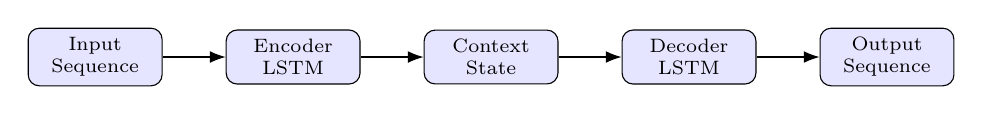
\begin{tikzpicture}[node distance=8mm]
\node[layer](a){Input\\Sequence};
\node[layer,right=of a](b){Encoder\\LSTM};
\node[layer,right=of b](c){Context\\State};
\node[layer,right=of c](d){Decoder\\LSTM};
\node[layer,right=of d](e){Output\\Sequence};

\foreach \x/\y in {a/b,b/c,c/d,d/e}
\draw[arrow](\x)--(\y);
\end{tikzpicture}
\end{center}

The encoder converts the input sequence into a learned representation.
The decoder generates the output sequence one element at a time.

\result{\textbf{Observed setup.} Sequences of length 6 were generated with integer tokens in $\{1,\dots,20\}$: 5600 training, 800 validation and 1600 test sequences. The model is an embedding (dimension 32) followed by an encoder LSTM and a decoder LSTM (64 units each) whose initial state is the encoder's final state, with a softmax output layer (52,631 parameters in total). It was trained with teacher forcing for 25 epochs (Adam, learning rate $10^{-3}$, batch size 64, 40.9 s); at test time the decoder generates the output greedily one token at a time. Evaluation used 300 test sequences.}

%%%%%%%%%%%%%%%%%%%%%%%%%%%%%%%%%%%%%%%%%%%%%%%%%%%%%%%%%%%%
\section*{23. Expected Sequence-to-Sequence Input and Output}

\textbf{Input example:}

\[
[3,8,1,5]
\]

\textbf{Expected output:}

\[
[5,1,8,3].
\]

Five test examples are shown below.

\begin{center}
\small
\begin{tabular}{|c|c|c|c|c|}
\hline
Sample & Input Sequence & Expected (reversed) & Predicted Output & Correct\\
\hline
1 & [15, 15, 18, 14, 1, 10] & [10, 1, 14, 18, 15, 15] & [10, 1, 14, 15, 18, 18] & No\\
2 & [15, 18, 7, 18, 16, 2] & [2, 16, 18, 7, 18, 15] & [2, 16, 18, 7, 18, 15] & Yes\\
3 & [12, 19, 12, 13, 1, 19] & [19, 1, 13, 12, 19, 12] & [19, 1, 13, 12, 19, 12] & Yes\\
4 & [4, 17, 19, 14, 10, 6] & [6, 10, 14, 19, 17, 4] & [6, 10, 14, 19, 17, 4] & Yes\\
5 & [17, 10, 2, 9, 2, 18] & [18, 2, 9, 2, 10, 17] & [18, 2, 9, 2, 10, 17] & Yes\\
\hline
\end{tabular}
\end{center}

%%%%%%%%%%%%%%%%%%%%%%%%%%%%%%%%%%%%%%%%%%%%%%%%%%%%%%%%%%%%
\section*{24. Sequence-to-Sequence Evaluation}

The following quantities are reported:

\begin{itemize}
\item Token accuracy
\item Sequence accuracy
\item Training loss
\item Validation loss
\end{itemize}

Token accuracy is

\[
\text{Token Accuracy}
=
\frac{\text{Correctly predicted tokens}}
{\text{Total tokens}}.
\]

Sequence accuracy is

\[
\text{Sequence Accuracy}
=
\frac{\text{Completely correct sequences}}
{\text{Total sequences}}.
\]



\result{\textbf{Observed results (300 test sequences).}
\begin{center}
\begin{tabular}{|l|c|}
\hline
Metric & Value\\
\hline
Token accuracy & 98.50\%\\
Sequence accuracy & 97.67\%\\
Final training loss & 0.0315\\
Final validation loss & 0.0404\\
\hline
\end{tabular}
\end{center}}

\figtwo{images/plot2_seq2seq_loss.png}{images/plot3_seq2seq_accuracy.png}{Sequence-to-sequence reversal: training/validation loss (left) and token accuracy (right) over 25 epochs.}{fig:s2s}

\result{\textbf{Inference.} Training loss falls from 2.79 to 0.031 and validation loss from 2.44 to 0.040, with validation token accuracy reaching 99.6\%: the encoder--decoder learns the reversal, and the small train/validation gap indicates no significant overfitting. Sequence accuracy can never exceed token accuracy, because one wrong token makes a whole sequence wrong. Here they are close (98.50\% vs 97.67\%) because the errors are concentrated: 97.67\% of 300 sequences is 293 correct, so 7 sequences contain all the errors, i.e. about 27 wrong tokens out of 1800 (about four wrong tokens per failed sequence, derived from the reported percentages assuming six tokens per sequence). With longer sequences, or with independent per-token errors, the gap would widen, since the probability that all $L$ tokens are correct is roughly $p^{L}$. The one failed example in the table above (input $[15,15,18,14,1,10]$) contains the repeated tokens 15 and 18, and the prediction has the right multiset of tokens in the wrong order for the repeated values, suggesting that repeated tokens are the hardest case for the decoder (a hypothesis based on one example).}

%%%%%%%%%%%%%%%%%%%%%%%%%%%%%%%%%%%%%%%%%%%%%%%%%%%%%%%%%%%%
\section*{25. Consolidated Results}

\begin{center}
\begin{tabular}{|l|c|c|c|c|c|}
\hline
Model & Accuracy & Precision & Recall & F1 & Parameters\\
\hline
RNN (HAR) & 69.29 & 68.99 & 68.49 & 68.02 & 1,974\\
LSTM (HAR) & 89.11 & 89.11 & 89.30 & 89.16 & 6,006\\
GRU (HAR) & 89.55 & 89.55 & 89.70 & 89.50 & 4,758\\
CNN--LSTM (video) & 100.00 & 100.00 & 100.00 & 100.00 & 168,229\\
CNN--GRU (video) & 87.50 & 93.33 & 90.00 & 89.33 & 126,309\\
\hline
\end{tabular}
\end{center}

All values are percentages except the parameter count; the HAR rows use the 2947-window test set and the video rows the 8-video test set.

Sequence-to-sequence task:

\begin{center}
\begin{tabular}{|l|c|c|c|c|c|}
\hline
Task & Token Acc. (\%) & Sequence Acc. (\%) & Train Loss & Val Loss & Parameters\\
\hline
Sequence reversal & 98.50 & 97.67 & 0.0315 & 0.0404 & 52,631\\
\hline
\end{tabular}
\end{center}

%%%%%%%%%%%%%%%%%%%%%%%%%%%%%%%%%%%%%%%%%%%%%%%%%%%%%%%%%%%%
\section*{26. Discussion Questions}

\begin{enumerate}[itemsep=6pt,topsep=3pt]
\item \textbf{What is a recurrent neural network?}\par\smallskip
A recurrent neural network (RNN) is a network for sequential data that processes a sequence one element at a time and carries a hidden state from one step to the next: $h_t=\tanh(W_xx_t+W_hh_{t-1}+b_h)$. The same weights are reused at every time step, so the number of parameters does not depend on the sequence length (the RNN used here has 1,974 parameters for $T=128$), and the output at step $t$ depends on the whole history $x_1,\dots,x_t$ through $h_t$.

\item \textbf{What information is represented by the hidden state?}\par\smallskip
The hidden state is a fixed-size vector (32-dimensional here) that summarizes, in a lossy and learned way, the information in the inputs seen so far that is useful for the task. It acts as the network's short-term memory: it is combined with the next input to give the next state and, for classification, the final state $h_T$ is passed to the classifier. In an LSTM, $h_t$ is the exposed output of a separate, longer-lived cell state $C_t$.

\item \textbf{Why is sequence order important?}\par\smallskip
The meaning of a sequence depends on the order and timing of its elements; the same values in a different order form a different, often meaningless, sequence. In the HAR signals, the gait rhythm and the phase relation between accelerometer and gyroscope peaks (Plot 1) identify walking, and shuffling the 128 time steps would destroy them. In the seq2seq task, reversal is defined entirely by order.

\item \textbf{Explain the difference between a feed-forward network and an RNN.}\par\smallskip
A feed-forward network maps a fixed-size input to an output with no memory and treats each input independently. To process a $128\times9$ window it would have to flatten it into 1152 features and learn separate weights for every time position, so a pattern learned at one position would not transfer to another and the parameter count would grow with $T$. An RNN has a recurrent connection $h_{t-1}\to h_t$, shares its weights across time, accepts sequences of any length and produces outputs that depend on past inputs; the price is sequential computation (time steps cannot be parallelized) and the need for BPTT.

\item \textbf{Explain Backpropagation Through Time.}\par\smallskip
BPTT is backpropagation applied to the RNN unrolled over $T$ steps, treating it as a deep network whose layers share the same weights. The gradient with respect to a shared weight is the sum of its contributions from all time steps:
\[
\frac{\partial L}{\partial W_h}=\sum_{t}\sum_{k\le t}\frac{\partial L}{\partial h_t}\Bigl(\prod_{j=k+1}^{t}\frac{\partial h_j}{\partial h_{j-1}}\Bigr)\frac{\partial^{+}h_k}{\partial W_h},
\qquad
\frac{\partial h_j}{\partial h_{j-1}}=\mathrm{diag}(1-h_j^{2})\,W_h,
\]
where $\partial^{+}$ is the immediate derivative. Time and memory cost grow linearly with $T$; truncated BPTT limits the number of unrolled steps.

\item \textbf{Why can gradients vanish during BPTT?}\par\smallskip
The gradient reaching step $k$ contains a product of $t-k$ Jacobians $\mathrm{diag}(1-h_j^2)W_h$. Since $|\tanh'|\le1$, if the largest singular value of $W_h$ is below 1 the norm of this product decays exponentially in $t-k$, so early inputs receive almost no gradient and the network cannot learn dependencies over many steps. This is consistent with our results: the vanilla RNN reaches only about 77\% training accuracy and is unstable across seeds (test F1 $72.9\pm7.0$\% at $T{=}128$ over three seeds, against $89.3\pm1.0$\% for the LSTM). The single-seed decline from 70.8\% to 67.7\% as $T$ grows from 32 to 128 is within that instability and is not evidence by itself; the cause was not measured directly (for example by gradient norms).

\item \textbf{Why can gradients explode during BPTT?}\par\smallskip
If the Jacobians in the same product are repeatedly larger than 1 in norm (a necessary condition is that the spectral radius of $W_h$ exceeds 1), the product grows exponentially, giving very large gradients, unstable updates and loss spikes or NaNs. It is mitigated by gradient-norm clipping, careful (e.g.\ orthogonal) initialization and a smaller learning rate.

\item \textbf{What are long-term dependencies?}\par\smallskip
Long-term dependencies are cases in which the correct output at time $t$ depends on an input that occurred many steps earlier ($t-k$ large), so information must be stored over a long interval and gradients must flow across it. Vanilla RNNs handle them poorly because of vanishing gradients; gated architectures were introduced to address this.

\item \textbf{What is the role of the LSTM cell state?}\par\smallskip
The cell state $C_t=f_tC_{t-1}+i_t\tilde{C}_t$ is the LSTM's long-term memory. Because it is updated additively and $\partial C_t/\partial C_{t-1}=\mathrm{diag}(f_t)$, information and gradients can flow over many steps without repeated squashing by $\tanh$ or multiplication by $W_h$ when $f_t\approx1$ (the ``constant error carousel''), which mitigates vanishing gradients. It is kept separate from the output $h_t$, so the cell can store information that is not exposed at every step.

\item \textbf{What are the forget, input and output gates in LSTM?}\par\smallskip
The forget gate $f_t=\sigma(W_f[h_{t-1},x_t]+b_f)$ decides how much of the previous cell state is kept (0 erases, 1 keeps); the input gate $i_t$ decides how much of the new candidate $\tilde{C}_t$ is written into the cell; the output gate $o_t$ decides how much of $\tanh(C_t)$ is exposed as the hidden state $h_t$. Each is a vector of values in $(0,1)$ computed from $h_{t-1}$ and $x_t$ and acts as a learned soft switch on each memory component.

\item \textbf{What are the reset and update gates in GRU?}\par\smallskip
The update gate $z_t$ controls how much of the state is overwritten: $h_t=(1-z_t)h_{t-1}+z_t\tilde{h}_t$, so $z_t\approx0$ copies the old state unchanged (an additive shortcut like the LSTM cell state). The reset gate $r_t$ controls how much of the previous state is used to compute the candidate $\tilde{h}_t=\tanh(W_h[r_t\odot h_{t-1},x_t]+b_h)$; $r_t\approx0$ lets the unit ignore the past and start afresh.

\item \textbf{Compare LSTM and GRU.}\par\smallskip
Both are gated recurrent units with an additive state path. The LSTM has a separate cell state and hidden state, three gates and four weight blocks; the GRU merges cell and hidden state, has two gates and three weight blocks, and therefore has fewer parameters (4,128 vs 5,376 in the recurrent layer here; 4,758 vs 6,006 in the full models, i.e.\ 20.8\% fewer). The LSTM's output gate can hide memory content, whereas the GRU exposes its whole state. Empirically they were indistinguishable here (test macro F1 89.16\% vs 89.50\%; LSTM better at $T{=}64$, 91.56\% vs 89.79\%; GRU marginally better at $T{=}32$, 86.80\% vs 86.43\%), in line with published comparisons that find no consistent winner. The GRU is attractive when parameters and latency matter; the LSTM when its extra memory control is useful.

\item \textbf{Why does GRU generally use a simpler gating mechanism than LSTM?}\par\smallskip
The GRU (Cho et al., 2014) was designed to keep the benefit of gating with less computation: it removes the separate cell state and the output gate and couples ``forget'' and ``input'' into one update gate (the weights $1-z_t$ and $z_t$ sum to one). This reduces the number of gates from three to two and the number of weight blocks from four to three, while preserving an additive path for information and gradients.

\item \textbf{Why should RNN, LSTM and GRU be compared using the same experimental settings?}\par\smallskip
A controlled comparison changes one factor only. If the models differed in data split, preprocessing, optimizer, learning rate, batch size, epochs, output layers or seed, a difference in performance could not be attributed to the recurrent cell. Here all three use the same windows, 32 units, dropout 0.2, the same Dense(16)--Dense(6) head, Adam ($10^{-3}$), batch size 32 and 30 epochs, so the differences can be attributed to the recurrent layer (although one seed per model still leaves a run-to-run variation of a few tenths of an F1 point).

\item \textbf{What does the confusion matrix reveal that accuracy alone does not?}\par\smallskip
Accuracy is a single number, whereas the confusion matrix shows which classes are confused with which, in which direction, and the per-class recall and precision. For example, the RNN's 69.3\% accuracy hides a WALKING recall of only 32.9\% against 95.0\% for LAYING, and the roughly 89\% accuracy of the LSTM and GRU hides that most of their errors are SITTING$\leftrightarrow$STANDING confusions (104 and 95 windows for the LSTM).

\item \textbf{Why should macro F1-score be reported for multi-class classification?}\par\smallskip
Macro F1 computes the F1-score (the harmonic mean of precision and recall) separately for each class and averages the results with equal weight, so every class counts equally regardless of its number of samples. Accuracy is dominated by frequent classes and can be high even if a rare class is never recognized, while F1 penalizes a model whose precision and recall are unbalanced. Here the classes are nearly balanced, so macro F1 and accuracy are close (89.16\% vs 89.11\% for the LSTM), but macro F1 is the safer summary.

\item \textbf{What is the significance of sequence length?}\par\smallskip
The sequence length determines how much temporal context the model sees (128 steps at 50~Hz is 2.56~s), the depth of the unrolled network, and the computation per sequence (linear in $T$). Too little context makes activities ambiguous (LSTM F1 86.4\% at $T{=}32$ vs 91.6\% at $T{=}64$), whereas longer sequences make optimization harder for the vanilla RNN (which is unstable at $T{=}128$: F1 $72.9\pm7.0$\% over three seeds; the single-seed trend 70.8\% $\to$ 67.7\% is within that noise) and cost more computation.

\item \textbf{Why can a CNN be used as a feature extractor for video?}\par\smallskip
Video frames are images, for which CNNs are the appropriate feature extractors. A CNN pretrained on ImageNet has learned a hierarchy of generic features (edges, textures, parts, objects) that transfers to new datasets, reduces a $224\times224\times3$ frame (150,528 values) to a 1280-dimensional descriptor, and can be run once and cached. With only 40 videos, training a CNN from scratch would overfit; keeping it frozen leaves only the small recurrent classifier to train.

\item \textbf{What type of information is extracted by the CNN?}\par\smallskip
The CNN extracts spatial, per-frame information: the appearance of the scene and objects, textures, colours and the shapes and configuration of people and objects (e.g.\ a court, a bicycle, a dog). Each frame is processed independently, so the CNN captures no temporal information.

\item \textbf{What type of information is learned by the recurrent network?}\par\smallskip
The recurrent network learns temporal information: how the frame descriptors change across the ten sampled frames (motion and its order, e.g.\ the trajectory of a dunk or the cyclic motion of pedalling), and it integrates this evidence over time into a single video-level decision.

\item \textbf{Why are CNN features arranged as a sequence before being given to LSTM/GRU?}\par\smallskip
LSTM/GRU layers take input of shape (batch, time, features) and consume one feature vector per time step, in order. Placing the per-frame CNN descriptors in chronological order gives a $10\times1280$ sequence, so the recurrent state can model how the content changes from one frame to the next. Averaging the descriptors or presenting them unordered would discard this temporal structure.

\item \textbf{Explain the encoder and decoder in sequence-to-sequence learning.}\par\smallskip
The encoder (an LSTM) reads the input sequence and compresses it into a fixed-size context, its final hidden and cell states (64 units each). The decoder (another LSTM) is initialized with this context and generates the output sequence one element at a time: at each step it receives the previous output token and its state and produces a softmax distribution over the vocabulary, until the sequence is complete. This allows input and output to have different lengths; the main limitation is the fixed-size bottleneck, which attention mechanisms relieve.

\item \textbf{What is teacher forcing?}\par\smallskip
In teacher forcing the decoder input at step $t$ during training is the ground-truth token of step $t-1$ instead of the model's own previous prediction. This makes training faster and more stable and lets all time steps be computed in parallel, but it creates a train/test mismatch (exposure bias): at inference the decoder must feed back its own predictions, so an early error can propagate. In this experiment the model was trained with teacher forcing and decoded greedily at test time.

\item \textbf{Differentiate token accuracy and sequence accuracy.}\par\smallskip
Token accuracy is the fraction of individual output tokens that are correct; sequence accuracy is the fraction of sequences in which every token is correct, so it can never exceed token accuracy. If errors were independent with token accuracy $p$, the sequence accuracy for length-$L$ outputs would be about $p^{L}$, i.e.\ $0.985^{6}\approx91.3\%$ here. The measured sequence accuracy is 97.67\% (vs.\ 98.50\% token accuracy) because the errors are concentrated in a few sequences (7 of 300); for longer sequences or less concentrated errors the gap becomes large.

\item \textbf{Why must the test set remain untouched during model selection?}\par\smallskip
If the test set is used to select models or tune hyperparameters, information about it leaks into the model, so the reported test score becomes optimistically biased and no longer estimates performance on unseen data. Selection and tuning must use the validation set, and the test set is used once for the final report. In this experiment the settings were fixed in advance and the test set was used only for the final evaluation.
\end{enumerate}

%%%%%%%%%%%%%%%%%%%%%%%%%%%%%%%%%%%%%%%%%%%%%%%%%%%%%%%%%%%%
\section*{27. Additional Exercises}

The notebook contains no code for these seven exercises. They were therefore run separately, with a re-implementation of the notebook pipeline (same data subset and split, same normalization fitted on the training windows, Adam with learning rate $10^{-3}$, batch size 32, 30 epochs, dropout 0.2, Dense(16)--Dense(6) head; code and raw per-run results are in the folder \texttt{additional\_exercises}).

\textbf{Protocol and how to read the numbers.} The seed-42 vanilla RNN results in Sections 14--17 turned out to be unrepresentative (its test F1 varies by up to 14 points between seeds, Exercise~1), so every HAR configuration below was trained with three seeds (42, 43, 44; the seed changes the weight initialization and batch order, not the data split) and is reported as mean$\pm$sample standard deviation with $n=3$. A standard deviation from three runs is itself uncertain, so differences smaller than about one standard deviation are treated as \emph{not established}. The test set has 2,947 windows, so even for a single fixed model the binomial standard error of an accuracy near 90\% is about 0.6 points. Training times in Exercises 1--4 and 7 come from a different CPU-only machine than Section 14 and are comparable with one another but not with Section 14; on that machine the seed-42 LSTM configuration gave 88.09\% accuracy rather than the notebook's 89.16\%, so runs are not bit-reproducible across machines. The three-seed means for the 32-unit baselines (LSTM 89.27\%, GRU 89.91\%, RNN 72.94\% F1) are consistent with the main experiment for the LSTM and GRU; the main experiment's RNN value (68.0\%) lies inside the RNN's seed range (65.8--79.8\%).

%%%%
\subsection*{Exercise 1 --- 16, 32 and 64 recurrent units}
\textit{Replace the 32 recurrent units with 16 and 64 units and study the effect on accuracy, F1-score, parameter count and training time.}

\begin{center}\small
\begin{tabular}{|l|c|r|c|c|c|}
\hline
Model & Units & Params & Accuracy (\%) & Macro-F1 (\%) & Train time (s)\\
\hline
RNN & 16 & 790 & 66.93$\pm$2.31 & 65.20$\pm$2.62 & 38.8$\pm$3.2\\
RNN & 32 & 1,974 & 74.10$\pm$5.97 & 72.94$\pm$7.01 & 40.1$\pm$0.7\\
RNN & 64 & 5,878 & 73.24$\pm$6.68 & 72.59$\pm$7.20 & 41.2$\pm$2.4\\
\hline
LSTM & 16 & 2,038 & 87.81$\pm$1.53 & 87.72$\pm$1.54 & 65.6$\pm$3.4\\
LSTM & 32 & 6,006 & 89.24$\pm$1.00 & 89.27$\pm$1.01 & 66.3$\pm$1.4\\
LSTM & 64 & 20,086 & 90.54$\pm$0.63 & 90.55$\pm$0.62 & 85.5$\pm$20.4\\
\hline
GRU & 16 & 1,670 & 88.84$\pm$1.17 & 88.74$\pm$1.10 & 82.2$\pm$4.6\\
GRU & 32 & 4,758 & 89.82$\pm$0.44 & 89.91$\pm$0.39 & 88.7$\pm$2.0\\
GRU & 64 & 15,542 & 90.53$\pm$1.09 & 90.53$\pm$1.08 & 120.7$\pm$7.7\\
\hline
\end{tabular}
\end{center}

\figone{images/ex1_units.png}{0.98}{Exercise 1: test macro-F1 (left) and 30-epoch training time (right) versus the number of recurrent units; mean and standard deviation over three seeds.}{fig:ex1}

\result{\textbf{Inference (Exercise 1).}
\textit{LSTM and GRU.} Macro-F1 increases with width: LSTM 87.7 $\to$ 89.3 $\to$ 90.6\% and GRU 88.7 $\to$ 89.9 $\to$ 90.5\% for 16 $\to$ 32 $\to$ 64 units. The 16$\to$64 gain has the same sign in all three seeds for both cells (LSTM $+4.5$, $+2.4$, $+1.6$; GRU $+1.9$, $+1.7$, $+1.8$ points), so it is unlikely to be noise, whereas the individual 16$\to$32 and 32$\to$64 steps (about 0.6--1.6 points) are of the same size as the seed standard deviation. Returns diminish: the parameter count grows roughly quadratically with the width because of the $h\times h$ recurrent matrices (LSTM 2,038 $\to$ 20,086, i.e.\ 9.9$\times$; GRU 1,670 $\to$ 15,542, 9.3$\times$), while the 32$\to$64 step buys only $+1.3$ (LSTM) and $+0.6$ (GRU) F1 points for 3.3$\times$ the parameters. Around 32 units is the knee of the curve for this task.
\textit{Vanilla RNN.} The RNN shows no reliable dependence on width: $65.2 \to 72.9 \to 72.6$\% with standard deviations of 2.6, 7.0 and 7.2 points; the per-seed F1 at 32 units ranges from 65.8 to 79.8\%. Only the lower value at 16 units is consistent across seeds (all three seeds improve from 16 to 32 units). Even the best RNN mean is far below the worst LSTM/GRU mean (87.7\%), and quadrupling the width does not close the gap, so the RNN's problem is optimization stability, not capacity. Vanishing or exploding gradients over 128 steps are the usual explanation and are consistent with this behaviour, but we did not measure gradient norms or test clipping, so this remains a hypothesis.
\textit{Training time.} The RNN's time is flat (38.8 $\to$ 41.2~s): with tiny matrix products, the cost is dominated by the sequential loop over 128 steps and by framework overhead rather than by arithmetic. The LSTM is flat from 16 to 32 units (65.6, 66.3~s) and then rises (85.5~s, but with a large spread of $\pm20$~s because one seed took 108.8~s on the shared machine); the GRU rises steadily (82.2, 88.7, 120.7~s). Timings are therefore approximate; the reliable statement is that cost grows slowly with width until the matrix products become large enough to matter.}

%%%%
\subsection*{Exercise 2 --- GRU versus LSTM with the same number of units}
\textit{Compare GRU and LSTM using the same number of recurrent units.}

\begin{center}\footnotesize\setlength{\tabcolsep}{4pt}
\begin{tabular}{|c|r|r|c|c|c|c|c|}
\hline
Units & Params LSTM & Params GRU & $\Delta$ params & F1 LSTM (\%) & F1 GRU (\%) & $\Delta$F1, GRU$-$LSTM & Time GRU/ LSTM\\
\hline
16 & 2,038 & 1,670 & -18\% & 87.72$\pm$1.54 & 88.74$\pm$1.10 & +1.02 (+2.8, +2.1, -1.9) & 1.25$\times$\\
32 & 6,006 & 4,758 & -21\% & 89.27$\pm$1.01 & 89.91$\pm$0.39 & +0.64 (+1.5, +0.4, -0.0) & 1.34$\times$\\
64 & 20,086 & 15,542 & -23\% & 90.55$\pm$0.62 & 90.53$\pm$1.08 & -0.02 (+0.2, +1.4, -1.7) & 1.41$\times$\\
\hline
\end{tabular}
\end{center}

\result{\textbf{Inference (Exercise 2).}
At equal width the GRU has 18--23\% fewer parameters (three gate/candidate blocks instead of four; the GRU's smaller size is exact by construction) but its accuracy is not distinguishable from the LSTM's: the mean F1 difference is $+1.0$, $+0.6$ and $0.0$ points at 16, 32 and 64 units, its sign is not consistent across seeds (e.g.\ $+2.8$, $+2.1$, $-1.9$ at 16 units), and the standard deviations are 0.4--1.5 points. The GRU is nominally ahead at small widths and the gap closes at 64 units, which fits the idea that the GRU makes more efficient use of a small state, but three seeds cannot establish this. The single-seed sequence-length results of Section~17 give the same picture ($T{=}32$: GRU $+0.4$; $T{=}64$: $-1.8$; $T{=}128$: $-0.2$ F1 points). A fair conclusion is that, on this task, the two cells reach the same accuracy and the GRU does so with about one fifth fewer parameters.
The \emph{time} ordering is, in contrast, consistent: the GRU is slower than the LSTM in every seed and at every width, by 1.25$\times$, 1.34$\times$ and 1.41$\times$ in the recorded runs and by 1.27--1.44$\times$ in the interleaved benchmark of Exercise~5. This is the opposite of what the parameter count suggests. We did not profile the cause. It is a property of this Keras/CPU implementation (for instance of how the GRU's gate matrices are evaluated) and need not hold on other hardware or backends, so it should not be read as an intrinsic disadvantage of the GRU.}

%%%%
\subsection*{Exercise 3 --- a second recurrent layer}
\textit{Add a second recurrent layer and investigate whether performance improves.}

The first recurrent layer returns its full sequence of hidden states, which the second recurrent layer (also 32 units) consumes; the rest of the model is unchanged.

\begin{center}\small
\begin{tabular}{|l|r|c|c|c|c|c|}
\hline
Model (32 units per layer) & Params & Accuracy (\%) & Macro-F1 (\%) & $\Delta$F1 & Train time (s) & Time ratio\\
\hline
RNN, 1 layer & 1,974 & 74.10$\pm$5.97 & 72.94$\pm$7.01 & -- & 40.1$\pm$0.7 & --\\
RNN, 2 layers & 4,054 & 69.09$\pm$9.64 & 66.92$\pm$11.95 & -6.02 & 80.7$\pm$3.2 & 2.0$\times$\\
\hline
LSTM, 1 layer & 6,006 & 89.24$\pm$1.00 & 89.27$\pm$1.01 & -- & 66.3$\pm$1.4 & --\\
LSTM, 2 layers & 14,326 & 90.66$\pm$0.90 & 90.65$\pm$0.98 & +1.38 & 132.2$\pm$3.8 & 2.0$\times$\\
\hline
GRU, 1 layer & 4,758 & 89.82$\pm$0.44 & 89.91$\pm$0.39 & -- & 88.7$\pm$2.0 & --\\
GRU, 2 layers & 11,094 & 89.58$\pm$0.18 & 89.56$\pm$0.14 & -0.35 & 229.4$\pm$18.3 & 2.6$\times$\\
\hline
\end{tabular}
\end{center}

\result{\textbf{Inference (Exercise 3).}
A second layer does not give a reliable improvement. For the LSTM the mean F1 rises by 1.4 points (89.3 $\to$ 90.6\%), but the gain is positive in only two of three seeds ($+3.4$, $-0.3$, $+1.0$) and comparable to the seed standard deviation of about 1.0, at 2.4$\times$ the parameters (6,006 $\to$ 14,326) and 2.0$\times$ the training time; a single wider layer (64 units, 20,086 parameters) reached 90.6\% as well. For the GRU the second layer is slightly \emph{worse} ($-0.35$ points, negative in all three seeds, but tiny) at 2.3$\times$ the parameters and 2.6$\times$ the time. For the vanilla RNN the two-layer model has a mean of 66.9\% against 72.9\% and a standard deviation of 11.9 points (per-seed 77.7, 69.0, 54.1\%), i.e.\ deeper stacking made this unstable model more variable, not better; the difference to the one-layer RNN is well within the noise. The HAR windows are short and the classes are separable by fairly simple temporal statistics, so extra depth has little to add, and it makes each epoch more expensive because the second layer must wait for the first layer's full output sequence. A deeper stack could help on harder data, and we did not tune dropout or learning rate per depth, which may favour the shallower models.}

%%%%
\subsection*{Exercise 4 --- bidirectional versus unidirectional LSTM}
\textit{Compare a bidirectional LSTM with a unidirectional LSTM.}

The bidirectional model wraps the 32-unit LSTM in \texttt{Bidirectional}, so the final forward and backward states (64 values in total) feed the same dropout and dense layers.

\begin{center}\small
\begin{tabular}{|l|r|c|c|c|c|}
\hline
Model (32 units) & Params & Accuracy (\%) & Macro-F1 (\%) & Precision / Recall (\%) & Train time (s)\\
\hline
LSTM & 6,006 & 89.24$\pm$1.00 & 89.27$\pm$1.01 & 89.25 / 89.41 & 66.3$\pm$1.4\\
Bidirectional LSTM & 11,894 & 89.42$\pm$1.69 & 89.46$\pm$1.71 & 89.52 / 89.63 & 79.9$\pm$2.1\\
\hline
\end{tabular}
\end{center}

\figone{images/ex3_ex4_depth.png}{0.72}{Exercises 3 and 4: test macro-F1 (mean$\pm$s.d., $n=3$) of one-layer, two-layer and bidirectional models with 32 units.}{fig:ex34}

\result{\textbf{Inference (Exercise 4).}
The bidirectional LSTM has almost twice the parameters (11,894 vs 6,006) and takes 1.2$\times$ as long, yet its F1 is $89.46\pm1.71$\% against $89.27\pm1.01$\%: a mean difference of $+0.19$ points with inconsistent sign ($+1.7$, $+1.1$, $-2.2$) and a larger spread. No benefit is demonstrated. This is the expected outcome for this problem: the whole 128-step window has one label and only the last hidden state is used, so the forward LSTM's final state has already seen every sample; the backward LSTM's final state sees the same samples in reverse order and adds little new information. Bidirectional layers pay off when the output at each position depends on \emph{future} context (tagging, per-frame labelling), not for one label per window. They are also unsuitable for real-time recognition because the backward pass needs the complete window before any output is available.}

%%%%
\subsection*{Exercise 5 --- sequence length and computational cost}
\textit{Change the sequence length and study the effect on computational cost.}

The recorded times are the 30-epoch training times of the sequence-length sweep in Section~17 (seed 42, notebook machine, checkpointing enabled). Because these single measurements are noisy, a controlled benchmark was added: each model is trained for 2 warm-up epochs, then timed for 15 further epochs (1,976 training windows, batch size 32), interleaving the nine configurations in every round so that machine-wide slow-downs affect all of them equally; the minimum over the 15 repeats is reported.

\begin{center}\small\setlength{\tabcolsep}{4pt}
\begin{tabular}{|c|c|c|c|c|c|c|c|}
\hline
 & & \multicolumn{3}{c|}{Recorded 30-epoch time (s)} & \multicolumn{3}{c|}{Benchmark: s per epoch (best of 15)}\\
\cline{3-8}
$T$ & Signal (s) & RNN & LSTM & GRU & RNN & LSTM & GRU\\
\hline
32 & 0.64 & 21.0 & 32.8 & 36.8 & 0.35 & 0.57 & 0.73\\
64 & 1.28 & 29.0 & 53.7 & 66.2 & 0.59 & 0.95 & 1.27\\
128 & 2.56 & 45.8 & 93.4 & 126.7 & 1.04 & 1.70 & 2.44\\
\hline
\multicolumn{2}{|c|}{Ratio $T{=}128$ / $T{=}32$} & 2.18$\times$ & 2.85$\times$ & 3.44$\times$ & 3.00$\times$ & 2.96$\times$ & 3.34$\times$\\
\hline
\end{tabular}
\end{center}

\figone{images/ex5_cost.png}{0.98}{Exercise 5: training time versus sequence length $T$ for the three cells; recorded 30-epoch times (left) and controlled benchmark (right).}{fig:ex5}

\result{\textbf{Inference (Exercise 5).}
The number of parameters does not depend on $T$ (RNN 1,974; LSTM 6,006; GRU 4,758) because the same weights are reused at every time step; $T$ changes the computation, which is sequential in $T$ (each step needs the previous hidden state, so it cannot be parallelized over time), and the memory needed to store activations for backpropagation through time (not measured here). Quadrupling $T$ from 32 to 128 increased the benchmarked epoch time by 3.0$\times$ (RNN), 3.0$\times$ (LSTM) and 3.3$\times$ (GRU), i.e.\ roughly linear but below 4$\times$ because part of each epoch (data feeding, the dense head, the optimizer step) does not depend on $T$. The recorded 30-epoch times agree in direction but scatter more (2.2$\times$, 2.9$\times$, 3.4$\times$). The benchmark itself showed bimodal epoch times (e.g.\ 0.35 s or 0.68 s for the same RNN, $T{=}32$ configuration), a sign of machine-level interference, which is why the minimum was used and why ratios below about 10\% should not be interpreted. The ordering RNN $<$ LSTM $<$ GRU holds at every $T$ (LSTM/RNN $\approx1.6\times$, GRU/LSTM 1.27$\times$ at $T{=}32$ rising to 1.44$\times$ at $T{=}128$).
Cost has to be weighed against accuracy (Section~17): for the LSTM, $T{=}64$ reached the highest single-seed F1 (91.6\%) at 56\% of the $T{=}128$ cost per epoch, while $T{=}32$ was cheaper still but 5 points worse. The $T{=}64$ versus $T{=}128$ difference (2.0 points) is about twice the LSTM seed standard deviation, so it is suggestive rather than established; what can be said is that doubling the window from 64 to 128 steps raised the cost per epoch by about 80\% without a measurable gain.}

%%%%
\subsection*{Exercise 6 --- LSTM versus GRU on identical CNN features}
\textit{For the video task, compare LSTM and GRU after extracting identical CNN features.}

The MobileNetV2 features saved for the notebook (40 real videos, 10 frames each, 1,280-dimensional) were reused unchanged, so both models see exactly the same inputs. Because the original test set contains only 8 videos, where one video is 12.5 accuracy points, a single split cannot separate the two cells. The comparison was therefore repeated over ten stratified 25/7/8 train/validation/test splits (seeds 0--9); in each split both models are trained with the notebook's settings (32 recurrent units, dropout 0.2, 20 epochs, no intermediate dense layer) and evaluated on the same 8 test videos.

\begin{center}\small
\begin{tabular}{|l|c|c|}
\hline
 & CNN--LSTM & CNN--GRU\\
\hline
Trainable parameters & 168,229 & 126,309\\
Test accuracy, mean$\pm$s.d.\ over 10 splits (\%) & 91.25$\pm$8.44 & 90.00$\pm$12.91\\
Test macro-F1, mean$\pm$s.d. (\%) & 92.00$\pm$7.95 & 88.53$\pm$14.81\\
Splits with 100\% test accuracy & 4 of 10 & 5 of 10\\
\hline
\end{tabular}
\end{center}
Paired difference in accuracy (GRU $-$ LSTM): -1.25 points (s.d.\ 10.94, standard error 3.46); the GRU was better in 2 splits, worse in 2 and tied in 6.

\figone{images/ex6_video.png}{0.45}{Exercise 6: test accuracy of CNN--LSTM and CNN--GRU in ten stratified splits (each marker is one split; markers at equal values are spread horizontally).}{fig:ex6}

\result{\textbf{Inference (Exercise 6).}
There is no evidence that either recurrent cell is better on identical features: the mean accuracies are 91.2\% (LSTM) and 90.0\% (GRU), and the paired difference of $-1.25$ points has a standard error of 3.5 points (approximate 95\% interval $\pm7.8$ points, and optimistic because the ten splits reuse the same 40 videos). The models differ by one or two test videos, in either direction, in four splits and are identical in six. The main experiment's 100\% (LSTM) versus 87.5\% (GRU) is therefore one video's worth of difference and lies inside this noise; it should not be reported as an advantage of the LSTM. The macro-F1 gap (92.0 vs 88.5\%) is driven mainly by two splits in which the GRU was much worse (62.5\% accuracy in one), only partly offset by two in which it was better, and is likewise not reliable. Both models reach 100\% training accuracy in every split, so the task at this size is limited by the tiny data set and apparently by the fact that the frozen CNN features already separate these five classes well, not by the recurrent cell. The GRU has 25\% fewer parameters (126,309 vs 168,229); a difference in accuracy smaller than roughly 10 points cannot be resolved with 8 test videos. Deciding between the cells for video would require a far larger test set (or a much harder class set).}

%%%%
\subsection*{Exercise 7 --- output sequence of a different length}
\textit{Modify the seq2seq task so that the output sequence has a different length from the input sequence.}

The encoder--decoder of Sections 22--24 was left unchanged (same layers and hyper-parameters, 8,000 random sequences over the tokens 1--20, 5,600/800/1,600 for training/validation/test, 25 epochs, batch size 64, greedy decoding). Only the target construction and the maximum decoding length changed. Two tasks with a different output length were defined next to the notebook's control task: \emph{reverse and keep the first three} (6 tokens in, 3 out; the shorter output is the last three input tokens in reverse order) and \emph{mirror} (4 tokens in, 8 out; the input followed by its reverse, e.g.\ $[2,15,14,19]\to[2,15,14,19,19,14,15,2]$).

\begin{center}\footnotesize\setlength{\tabcolsep}{4pt}
\begin{tabular}{|l|c|c|c|c|c|}
\hline
Task & In $\to$ out & Token acc.\ (\%) & Sequence acc.\ (\%) & Length acc.\ (\%) & Train / val loss\\
\hline
Reverse (control) & 6 $\to$ 6 & 98.77$\pm$0.83 & 95.60$\pm$3.78 & 99.12$\pm$0.57 & 0.027$\pm$0.003 / 0.043$\pm$0.018\\
Reverse, keep first 3 (shorter) & 6 $\to$ 3 & 100.00$\pm$0.00 & 100.00$\pm$0.00 & 100.00$\pm$0.00 & 0.006$\pm$0.000 / 0.007$\pm$0.000\\
Mirror: copy + reverse (longer) & 4 $\to$ 8 & 89.44$\pm$2.17 & 75.98$\pm$3.67 & 98.00$\pm$0.45 & 0.132$\pm$0.023 / 0.146$\pm$0.014\\
\hline
\end{tabular}
\end{center}
All three models have 52,631 parameters (embedding 32, encoder and decoder LSTM 64 units, softmax over 23 symbols): nothing in the weights depends on the sequence lengths. Test set: 1,600 sequences per task, three seeds. Length accuracy is the fraction of test sequences whose generated output has exactly the required length (i.e.\ the decoder emitted the end-of-sequence token at the right step).

\figone{images/ex7_s2s.png}{0.72}{Exercise 7: token, sequence and length accuracy of the three seq2seq tasks (mean$\pm$s.d., three seeds).}{fig:ex7}

Per-position accuracy (seed 42; sequence accuracy 97.6\% for the reverse task and 72.1\% for the mirror task in this run):

\begin{center}\small
\begin{tabular}{|l|c|c|c|c|c|c|c|c|}
\hline
Output position & 1 & 2 & 3 & 4 & 5 & 6 & 7 & 8\\
\hline
Mirror 4$\to$8 (copy: 1--4, reverse: 5--8) & 96.4 & 89.4 & 86.6 & 93.1 & 83.0 & 84.1 & 80.8 & 82.3\\
Reverse 6$\to$6 & 99.8 & 99.8 & 99.5 & 99.4 & 98.4 & 97.9 & -- & --\\
\hline
\end{tabular}
\end{center}

\result{\textbf{Inference (Exercise 7).}
The architecture handles different input and output lengths without modification, because the decoder generates tokens until it emits the end-of-sequence symbol, and it learned to do so: the output length was correct for 98--100\% of the sequences in all tasks, so the errors are content errors, not termination errors. The shorter task was solved perfectly (100\% at token and sequence level in all seeds), better than the control (98.8\% token, $95.6\pm3.8$\% sequence accuracy). It is the easiest because it only requires the last three input tokens, which the encoder's final state retains best. The longer output was clearly harder although the input is shorter: 89.4\% token accuracy and only $76.0\pm3.7$\% sequence accuracy. Training loss (0.13) and validation loss (0.15) are close, so the model is underfitted rather than overfitted at 25 epochs; more epochs or units might narrow the gap, which we did not test. In the seed-42 run accuracy is highest at the first output positions (96\% at position 1) and lower in the reversed half (81--84\%), and sequences that contain a repeated token are much harder than those without (mirror: 51.4\% vs 80.2\% sequence accuracy; reverse: 96.4\% vs 99.0\%). A plausible reason is that a decoder without attention must track its position inside a 64-unit state, and repeated tokens make positions ambiguous, but this was not tested (the repeated-token comparison is confounded by the fact that repeated tokens are more frequent in longer sequences). Overall, output length matters less than how much of the input must be held and re-emitted through the fixed-size context vector.}

%%%%
\subsection*{Summary of the additional exercises}
Across three seeds, the main conclusions of the notebook hold for the LSTM and GRU but with much less certainty for the vanilla RNN. (i) Gating matters far more than any other factor tested: the mean F1 of every LSTM/GRU configuration (87.7--90.6\%) is well above that of every vanilla RNN configuration (65--73\%), and the RNN's results are unstable (a spread of 14 F1 points between seeds for one layer, 24 for two layers), so single-seed RNN comparisons in Sections 14--17 should be read with this in mind. (ii) Width helps the gated cells modestly with diminishing returns beyond 32 units; depth and bidirectionality do not give a demonstrable gain on this task. (iii) LSTM and GRU are equal in accuracy within noise, while the GRU is smaller but, in this implementation, slower. (iv) Cost grows roughly linearly with sequence length, and $T{=}64$ offers a better cost--accuracy point than $T{=}128$ for the LSTM. (v) With 40 videos, no difference between LSTM and GRU on identical features can be established. (vi) For sequence-to-sequence learning, a different output length is easy to support, and the difficulty is governed by how much information must pass through the fixed context vector. \emph{Limitations:} $n=3$ seeds; a single dataset; a HAR validation split that is random over windows (not subject-wise) and used only for monitoring; timings from a shared CPU machine; and a video test set of 8 videos per split.

%%%%%%%%%%%%%%%%%%%%%%%%%%%%%%%%%%%%%%%%%%%%%%%%%%%%%%%%%%%%
\section*{28. Expected Outcome}

At the end of the experiment, students should be able to demonstrate the
complete sequence-learning pipeline:

\[
\boxed{
\text{Sequential Data}
\rightarrow
\text{Preprocessing}
\rightarrow
\text{RNN/LSTM/GRU}
\rightarrow
\text{Evaluation}
}
\]

and the video-understanding pipeline:

\[
\boxed{
\text{Video}
\rightarrow
\text{Frames}
\rightarrow
\text{CNN Features}
\rightarrow
\text{LSTM/GRU}
\rightarrow
\text{Action Prediction}
}
\]

They should also understand the encoder--decoder formulation:

\[
\boxed{
\text{Input Sequence}
\rightarrow
\text{Encoder}
\rightarrow
\text{Context}
\rightarrow
\text{Decoder}
\rightarrow
\text{Output Sequence}
}
\]

%%%%%%%%%%%%%%%%%%%%%%%%%%%%%%%%%%%%%%%%%%%%%%%%%%%%%%%%%%%%
\section*{29. References}

\begin{enumerate}
\item Ian Goodfellow, Yoshua Bengio and Aaron Courville,
\emph{Deep Learning}, MIT Press, 2016.

\item Sepp Hochreiter and Jürgen Schmidhuber,
``Long Short-Term Memory,'' \emph{Neural Computation}, 1997.

\item Kyunghyun Cho et al.,
``Learning Phrase Representations using RNN Encoder--Decoder for Statistical
Machine Translation,'' EMNLP, 2014.

\item Anguita et al.,
``A Public Domain Dataset for Human Activity Recognition Using Smartphones,''
ESANN, 2013.

\item Khurram Soomro, Amir Roshan Zamir and Mubarak Shah,
``UCF101: A Dataset of 101 Human Actions Classes From Videos in the Wild,''
2012.

\item TensorFlow Documentation:
\url{https://www.tensorflow.org}

\item Keras Documentation:
\url{https://keras.io}
\end{enumerate}

\end{document}
